% Options for packages loaded elsewhere
\PassOptionsToPackage{unicode}{hyperref}
\PassOptionsToPackage{hyphens}{url}
%
\documentclass[
  english,
]{book}
\usepackage{amsmath,amssymb}
\usepackage{lmodern}
\usepackage{ifxetex,ifluatex}
\ifnum 0\ifxetex 1\fi\ifluatex 1\fi=0 % if pdftex
  \usepackage[T1]{fontenc}
  \usepackage[utf8]{inputenc}
  \usepackage{textcomp} % provide euro and other symbols
\else % if luatex or xetex
  \usepackage{unicode-math}
  \defaultfontfeatures{Scale=MatchLowercase}
  \defaultfontfeatures[\rmfamily]{Ligatures=TeX,Scale=1}
\fi
% Use upquote if available, for straight quotes in verbatim environments
\IfFileExists{upquote.sty}{\usepackage{upquote}}{}
\IfFileExists{microtype.sty}{% use microtype if available
  \usepackage[]{microtype}
  \UseMicrotypeSet[protrusion]{basicmath} % disable protrusion for tt fonts
}{}
\makeatletter
\@ifundefined{KOMAClassName}{% if non-KOMA class
  \IfFileExists{parskip.sty}{%
    \usepackage{parskip}
  }{% else
    \setlength{\parindent}{0pt}
    \setlength{\parskip}{6pt plus 2pt minus 1pt}}
}{% if KOMA class
  \KOMAoptions{parskip=half}}
\makeatother
\usepackage{xcolor}
\IfFileExists{xurl.sty}{\usepackage{xurl}}{} % add URL line breaks if available
\IfFileExists{bookmark.sty}{\usepackage{bookmark}}{\usepackage{hyperref}}
\hypersetup{
  pdftitle={ReCentering Psych Stats: Psychometrics},
  pdfauthor={Lynette H Bikos, PhD, ABPP},
  pdflang={en},
  hidelinks,
  pdfcreator={LaTeX via pandoc}}
\urlstyle{same} % disable monospaced font for URLs
\usepackage{color}
\usepackage{fancyvrb}
\newcommand{\VerbBar}{|}
\newcommand{\VERB}{\Verb[commandchars=\\\{\}]}
\DefineVerbatimEnvironment{Highlighting}{Verbatim}{commandchars=\\\{\}}
% Add ',fontsize=\small' for more characters per line
\usepackage{framed}
\definecolor{shadecolor}{RGB}{248,248,248}
\newenvironment{Shaded}{\begin{snugshade}}{\end{snugshade}}
\newcommand{\AlertTok}[1]{\textcolor[rgb]{0.94,0.16,0.16}{#1}}
\newcommand{\AnnotationTok}[1]{\textcolor[rgb]{0.56,0.35,0.01}{\textbf{\textit{#1}}}}
\newcommand{\AttributeTok}[1]{\textcolor[rgb]{0.77,0.63,0.00}{#1}}
\newcommand{\BaseNTok}[1]{\textcolor[rgb]{0.00,0.00,0.81}{#1}}
\newcommand{\BuiltInTok}[1]{#1}
\newcommand{\CharTok}[1]{\textcolor[rgb]{0.31,0.60,0.02}{#1}}
\newcommand{\CommentTok}[1]{\textcolor[rgb]{0.56,0.35,0.01}{\textit{#1}}}
\newcommand{\CommentVarTok}[1]{\textcolor[rgb]{0.56,0.35,0.01}{\textbf{\textit{#1}}}}
\newcommand{\ConstantTok}[1]{\textcolor[rgb]{0.00,0.00,0.00}{#1}}
\newcommand{\ControlFlowTok}[1]{\textcolor[rgb]{0.13,0.29,0.53}{\textbf{#1}}}
\newcommand{\DataTypeTok}[1]{\textcolor[rgb]{0.13,0.29,0.53}{#1}}
\newcommand{\DecValTok}[1]{\textcolor[rgb]{0.00,0.00,0.81}{#1}}
\newcommand{\DocumentationTok}[1]{\textcolor[rgb]{0.56,0.35,0.01}{\textbf{\textit{#1}}}}
\newcommand{\ErrorTok}[1]{\textcolor[rgb]{0.64,0.00,0.00}{\textbf{#1}}}
\newcommand{\ExtensionTok}[1]{#1}
\newcommand{\FloatTok}[1]{\textcolor[rgb]{0.00,0.00,0.81}{#1}}
\newcommand{\FunctionTok}[1]{\textcolor[rgb]{0.00,0.00,0.00}{#1}}
\newcommand{\ImportTok}[1]{#1}
\newcommand{\InformationTok}[1]{\textcolor[rgb]{0.56,0.35,0.01}{\textbf{\textit{#1}}}}
\newcommand{\KeywordTok}[1]{\textcolor[rgb]{0.13,0.29,0.53}{\textbf{#1}}}
\newcommand{\NormalTok}[1]{#1}
\newcommand{\OperatorTok}[1]{\textcolor[rgb]{0.81,0.36,0.00}{\textbf{#1}}}
\newcommand{\OtherTok}[1]{\textcolor[rgb]{0.56,0.35,0.01}{#1}}
\newcommand{\PreprocessorTok}[1]{\textcolor[rgb]{0.56,0.35,0.01}{\textit{#1}}}
\newcommand{\RegionMarkerTok}[1]{#1}
\newcommand{\SpecialCharTok}[1]{\textcolor[rgb]{0.00,0.00,0.00}{#1}}
\newcommand{\SpecialStringTok}[1]{\textcolor[rgb]{0.31,0.60,0.02}{#1}}
\newcommand{\StringTok}[1]{\textcolor[rgb]{0.31,0.60,0.02}{#1}}
\newcommand{\VariableTok}[1]{\textcolor[rgb]{0.00,0.00,0.00}{#1}}
\newcommand{\VerbatimStringTok}[1]{\textcolor[rgb]{0.31,0.60,0.02}{#1}}
\newcommand{\WarningTok}[1]{\textcolor[rgb]{0.56,0.35,0.01}{\textbf{\textit{#1}}}}
\usepackage{longtable,booktabs,array}
\usepackage{calc} % for calculating minipage widths
% Correct order of tables after \paragraph or \subparagraph
\usepackage{etoolbox}
\makeatletter
\patchcmd\longtable{\par}{\if@noskipsec\mbox{}\fi\par}{}{}
\makeatother
% Allow footnotes in longtable head/foot
\IfFileExists{footnotehyper.sty}{\usepackage{footnotehyper}}{\usepackage{footnote}}
\makesavenoteenv{longtable}
\usepackage{graphicx}
\makeatletter
\def\maxwidth{\ifdim\Gin@nat@width>\linewidth\linewidth\else\Gin@nat@width\fi}
\def\maxheight{\ifdim\Gin@nat@height>\textheight\textheight\else\Gin@nat@height\fi}
\makeatother
% Scale images if necessary, so that they will not overflow the page
% margins by default, and it is still possible to overwrite the defaults
% using explicit options in \includegraphics[width, height, ...]{}
\setkeys{Gin}{width=\maxwidth,height=\maxheight,keepaspectratio}
% Set default figure placement to htbp
\makeatletter
\def\fps@figure{htbp}
\makeatother
\setlength{\emergencystretch}{3em} % prevent overfull lines
\providecommand{\tightlist}{%
  \setlength{\itemsep}{0pt}\setlength{\parskip}{0pt}}
\setcounter{secnumdepth}{5}
\usepackage{booktabs}
\ifxetex
  % Load polyglossia as late as possible: uses bidi with RTL langages (e.g. Hebrew, Arabic)
  \usepackage{polyglossia}
  \setmainlanguage[]{english}
\else
  \usepackage[main=english]{babel}
% get rid of language-specific shorthands (see #6817):
\let\LanguageShortHands\languageshorthands
\def\languageshorthands#1{}
\fi
\ifluatex
  \usepackage{selnolig}  % disable illegal ligatures
\fi
\usepackage[]{natbib}
\bibliographystyle{plainnat}

\title{ReCentering Psych Stats: Psychometrics}
\author{Lynette H Bikos, PhD, ABPP}
\date{}

\begin{document}
\maketitle

{
\setcounter{tocdepth}{1}
\tableofcontents
}
\hypertarget{book-cover}{%
\chapter*{BOOK COVER}\label{book-cover}}
\addcontentsline{toc}{chapter}{BOOK COVER}

\begin{figure}
\centering
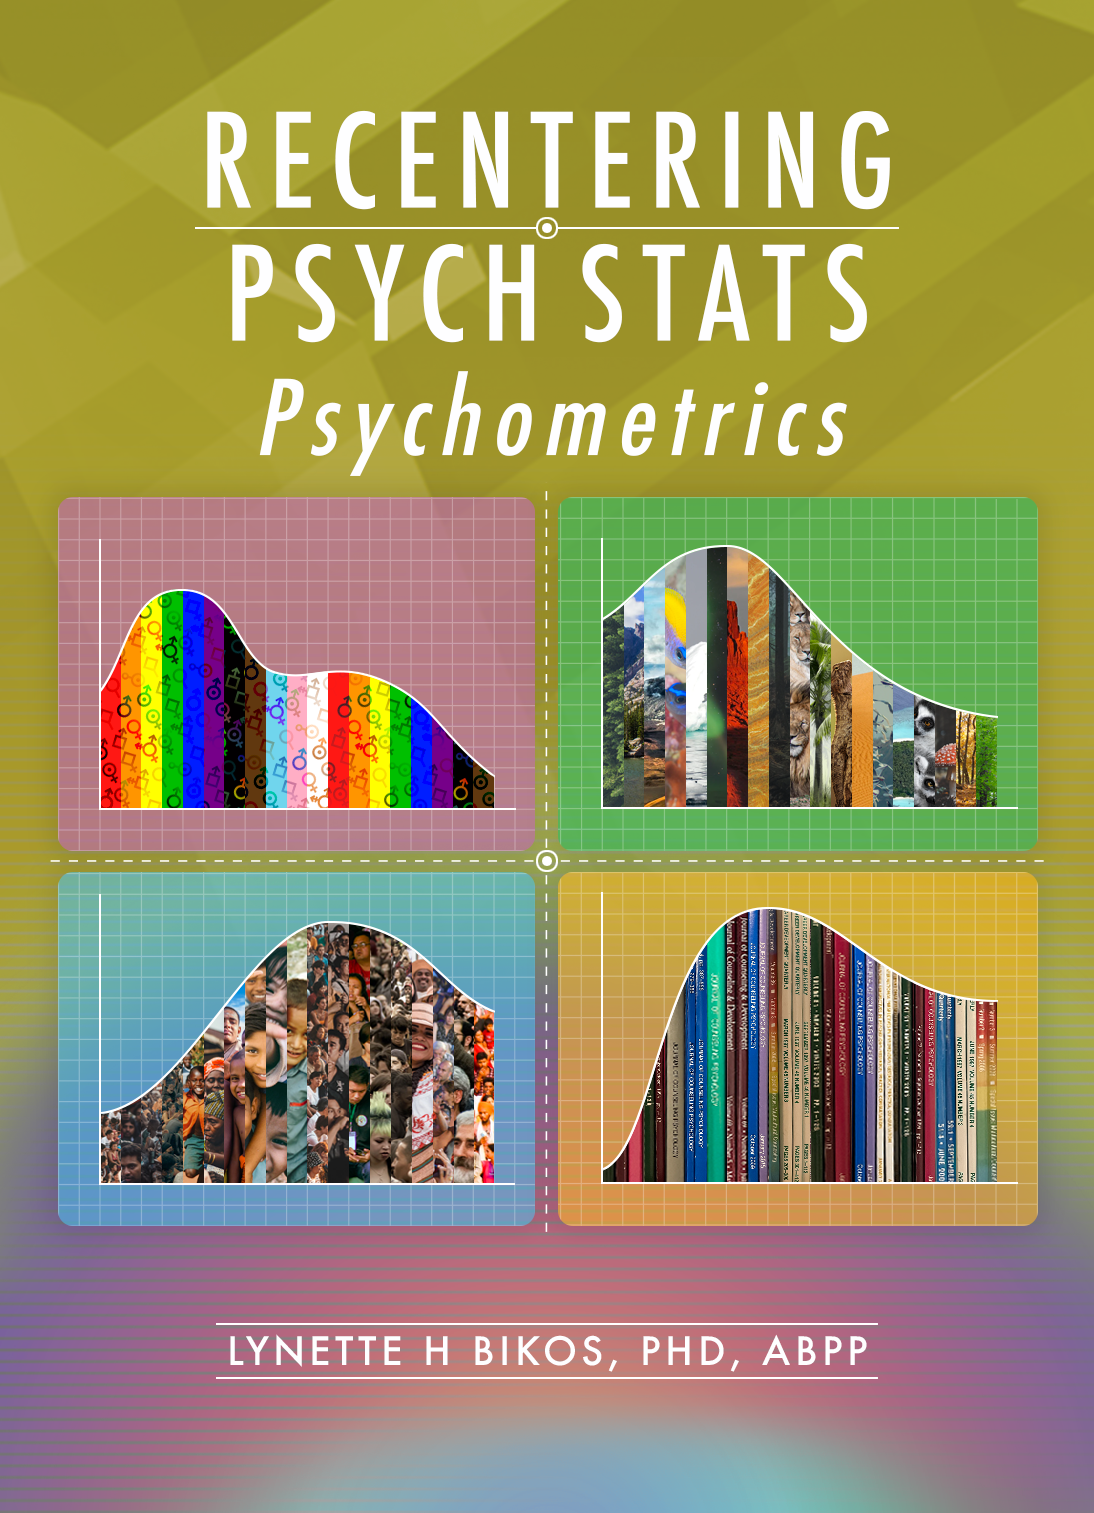
\includegraphics{images/ReCenterPsychStats-Psychometrics-bookcover.png}
\caption{An image of the book cover. It includes four quadrants of non-normal distributions representing gender, race/ethnicty, sustainability/global concerns, and journal articles}
\end{figure}

\hypertarget{preface}{%
\chapter*{Preface}\label{preface}}
\addcontentsline{toc}{chapter}{Preface}

\textbf{If you are viewing this document, you should know that this is a book-in-progress. Early drafts are released for the purpose teaching my classes and gaining formative feedback from a host of stakeholders. The document was last updated on 24 Aug 2021}. Emerging volumes on other statistics are posted on the \href{https://lhbikos.github.io/BikosRVT/ReCenter.html}{ReCentering Psych Stats} page at my research team's website.

\href{https://spu.hosted.panopto.com/Panopto/Pages/Viewer.aspx?id=c932455e-ef06-444a-bdca-acf7012d759a}{Screencasted Lecture Link}

To \emph{center} a variable in regression means to set its value at zero and interpret all other values in relation to this reference point. Regarding race and gender, researchers often center male and White at zero. Further, it is typical that research vignettes in statistics textbooks are similarly seated in a White, Western (frequently U.S.), heteronormative, framework. The purpose of this project is to create a set of open educational resources (OER) appropriate for doctoral and post-doctoral training that contribute to a socially responsive pedagogy -- that is, it contributes to justice, equity, diversity, and inclusion.

Statistics training in doctoral programs are frequently taught with fee-for-use programs (e.g., SPSS/AMOS, SAS, MPlus) that may not be readily available to the post-doctoral professional. In recent years, there has been an increase and improvement in R packages (e.g., \emph{psych}, \emph{lavaan}) used for in analyses common to psychological research. Correspondingly, many graduate programs are transitioning to statistics training in R (free and open source). This is a challenge for post-doctoral psychologists who were trained with other software. This OER will offer statistics training with R and be freely available (specifically in a GitHub respository and posted through GitHub Pages) under a Creative Commons Attribution - Non Commercial - Share Alike license {[}CC BY-NC-SA 4.0{]}.

Training models for doctoral programs in HSP are commonly scholar-practitioner, scientist-practitioner, or clinical-scientist. An emerging model, the \emph{scientist-practitioner-advocacy} training model incorporates social justice advocacy so that graduates are equipped to recognize and address the sociocultural context of oppression and unjust distribution of resources and opportunities \citep{mallinckrodt_scientist-practitioner-advocate_2014}. In statistics textbooks, the use of research vignettes engages the learner around a tangible scenario for identifying independent variables, dependent variables, covariates, and potential mechanisms of change. Many students recall examples in Field's \citeyearpar{field_discovering_2012} popular statistics text: Viagra to teach one-way ANOVA, beer goggles for two-way ANOVA, and bushtucker for repeated measures. What if the research vignettes were more socially responsive?

In this OER, research vignettes will be from recently published articles where:

\begin{itemize}
\tightlist
\item
  the author's identity is from a group where scholarship is historically marginalized (e.g., BIPOC, LGBTQ+, LMIC{[}low-middle income countries{]}),
\item
  the research is responsive to issues of justice, equity, inclusion, diversity,
\item
  the lesson's statistic is used in the article, and
\item
  there is sufficient information in the article to simulate the data for the chapter example(s) and practice problem(s); or it is publicly available.
\end{itemize}

In training for multicultural competence, the saying, ``A fish doesn't know that it's wet'' is often used to convey the notion that we are often unaware of our own cultural characteristics. In recent months and years, there has been an increased awakening to the institutional and systemic racism that our systems are perpetuating. Queuing from the water metaphor, I am hopeful that a text that is recentered in the ways I have described can contribute to \emph{changing the water} in higher education and in the profession of psychology.

\hypertarget{copyright-with-open-access}{%
\section*{Copyright with Open Access}\label{copyright-with-open-access}}
\addcontentsline{toc}{section}{Copyright with Open Access}

This book is published under a a Creative Commons Attribution-NonCommercial-ShareAlike 4.0 International License. This means that this book can be reused, remixed, retained, revised and redistributed (including commercially) as long as appropriate credit is given to the authors. If you remix, or modify the original version of this open textbook, you must redistribute all versions of this open textbook under the same license - CC BY-SA.

A \href{https://github.com/lhbikos/ReC_Psychometrics}{GitHub open-source repository} contains all of the text and source code for the book, including data and images.

\hypertarget{acknowledgements}{%
\chapter*{ACKNOWLEDGEMENTS}\label{acknowledgements}}
\addcontentsline{toc}{chapter}{ACKNOWLEDGEMENTS}

As a doctoral student at the University of Kansas (1992-2005), I learned that ``a foreign language'' was required for graduation. \emph{Please note that as one who studies the intersections of global, vocational, and sustainable psychology, I regret that I do not have language skills beyond English.} This could have been met with credit from high school my rural, mid-Missouri high school did not offer such classes. This requirement would have typically been met with courses taken during an undergraduate program -- but my non-teaching degree in the University of Missouri's School of Education was exempt from this. The requirement could have also been met with a computer language (fortran, C++) -- I did not have any of those either. There was a tiny footnote on my doctoral degree plan that indicated that a 2-credit course, ``SPSS for Windows'' would substitute for the language requirement. Given that it was taught by my one of my favorite professors, I readily signed up. As it turns out, Samuel B. Green, PhD, was using the course to draft chapters in the textbook \citep{green_using_2014} that has been so helpful for so many. Unfortunately, Drs. Green (1947 - 2018) and Salkind (2947 - 2017) are no longer with us. I have worn out numerous versions of their text. Another favorite text of mine was Dr.~Barbara Byrne's \citeyearpar{byrne_structural_2016}, ``Structural Equation Modeling with AMOS.'' I loved the way she worked through each problem and paired it with a published journal article, so that the user could see how the statistical evaluation fit within the larger project/article. I took my tea-stained text with me to a workshop she taught at APA and was proud of the signature she added to it (a little catfur might have fallen out). Dr.~Byrne created SEM texts for a number of statistical programs (e.g., LISREL, EQS, MPlus). As I was learning R, I wrote Dr.~Byrne, asking if she had an edition teaching SEM/CFA with R. She promptly wrote back, saying that she did not have the bandwidth to learn a new statistics package. We lost Dr.~Byrne in December 2020. I am so grateful to these role models for their contributions to my statistical training. I am also grateful for the doctoral students who have taken my courses and are continuing to provide input for how to improve the materials.

The inspiration for training materials that re*center statistics and research methods came from the \href{https://www.academics4blacklives.com/}{Academics for Black Survival and Wellness Initiative}. This project, co-founded by Della V. Mosley, Ph.D., and Pearis L. Bellamy, M.S., made clear the necessity and urgency for change in higher education and the profession of psychology.

At very practical levels, I am indebted to SPU's Library, and more specifically, SPU's Education, Technology, and Media Department. Assistant Dean for Instructional Design and Emerging Technologies, R. John Robertson, MSc, MCS, has offered unlimited consultation, support, and connection. Senior Instructional Designer in Graphics \& Illustrations, Dominic Wilkinson, designed the logo and bookcover. Psychology and Scholarly Communications Librarian, Kristin Hoffman, MLIS, has provided consultation on topics ranging from OERS to citations. I am alo indebted to Associate Vice President, Teaching and Learning at Kwantlen Polytechnic University, Rajiv Jhangiani, PhD. Dr.~Jhangiani's text \citeyearpar{jhangiani_research_2019} was the first OER I ever used and I was grateful for his encouraging conversation.

Financial support for this text has been provided from the \emph{Call to Action on Equity, Inclusion, Diversity, Justice, and Social Responsivity
Request for Proposals} grant from the Association of Psychology Postdoctoral and Internship Centers (2021-2022).

\hypertarget{ReCintro}{%
\chapter{Introduction}\label{ReCintro}}

\href{https://spu.hosted.panopto.com/Panopto/Pages/Viewer.aspx?pid=cc9b7c0d-e5c3-4e4e-a469-acf7013ee761}{Screencasted Lecture Link}

\hypertarget{what-to-expect-in-each-chapter}{%
\section{What to expect in each chapter}\label{what-to-expect-in-each-chapter}}

This textbook is intended as \emph{applied,} in that a primary goal is to help the scientist-practitioner-advocate use a variety of statistics in research problems and \emph{writing them up} for a program evaluation, dissertation, or journal article. In support of that goal, I try to provide just enough conceptual information so that the researcher can select the appropriate statistic (i.e., distinguishing between when ANOVA is appropriate and when regression is appropriate) and assign variables to their proper role (e.g., covariate, moderator, mediator).

This conceptual approach does include occasional, step-by-step, \emph{hand-calculations} (only we calculate them arithmetically in R) to provide a \emph{visceral feeling} of what is happening within the statistical algorithm that may be invisible to the researcher. Additionally, the conceptual review includes a review of the assumptions about the characteristics of the data and research design that are required for the statistic. Statistics can be daunting, so I have worked hard to establish a \emph{workflow} through each analysis. When possible, I include a flowchart that is referenced frequently in each chapter and assists the the researcher keep track of their place in the many steps and choices that accompany even the simplest of analyses.

As with many statistics texts, each chapter includes a \emph{research vignette.} Somewhat unique to this resource is that the vignettes are selected from recently published articles. Each vignette is chosen with the intent to meet as many of the following criteria as possible:

\begin{itemize}
\tightlist
\item
  the statistic that is the focus of the chapter was properly used in the article,
\item
  the author's identity is from a group where scholarship is historically marginalized (e.g., BIPOC, LGBTQ+, LMIC {[}low middle income countries{]}),
\item
  the research has a justice, equity, inclusion, diversity, and social responsivity focus and will contribute positively to a social justice pedagogy, and
\item
  the data is available in a repository or there is sufficient information in the article to simulate the data for the chapter example(s) and practice problem(s).
\end{itemize}

In each chapter we employ \emph{R} packages that will efficiently calculate the statistic and the dashboard of metrics (e.g., effect sizes, confidence intervals) that are typically reported in psychological science.

\hypertarget{strategies-for-accessing-and-using-this-oer}{%
\section{Strategies for Accessing and Using this OER}\label{strategies-for-accessing-and-using-this-oer}}

There are a number of ways you can access this resource. You may wish to try several strategies and then select which works best for you. I demonstrate these in the screencast that accompanies this chapter.

\begin{enumerate}
\def\labelenumi{\arabic{enumi}.}
\tightlist
\item
  Simply follow along in the .html formatted document that is available on via GitHug Pages, and then

  \begin{itemize}
  \tightlist
  \item
    open a fresh .rmd file of your own, copying (or retyping) the script and running it
  \end{itemize}
\item
  Locate the original documents at the \href{https://github.com/lhbikos/ReC_Psychometrics}{GitHub repository} . You can

  \begin{itemize}
  \tightlist
  \item
    open them to simply take note of the ``behind the scenes'' script
  \item
    copy/download individual documents that are of interest to you
  \item
    fork a copy of the entire project to your own GitHub site and further download it (in its entirety) to your personal workspace. The \href{https://desktop.github.com/}{GitHub Desktop app} makes this easy!
  \end{itemize}
\item
  Listen to the accompanying lectures (I think sound best when the speed is 1.75). The lectures are being recorded in Panopto and should include the closed captioning.
\item
  Provide feedback to me! If you fork a copy to your own GitHub repository, you can

  \begin{itemize}
  \tightlist
  \item
    open up an editing tool and mark up the document with your edits,
  \item
    start a discussion by leaving comments/questions, and then
  \item
    sending them back to me by committing and saving. I get an e-mail notiying me of this action. I can then review (accepting or rejecting) them and, if a discussion is appropriate, reply back to you.
  \end{itemize}
\end{enumerate}

\hypertarget{if-you-are-new-to-r}{%
\section{If You are New to R}\label{if-you-are-new-to-r}}

R can be oveRwhelming. Jumping right into advanced statistics might not be the easiest way to start. However, in these chapters, I provide complete code for every step of the process, starting with uploading the data. To help explain what R script is doing, I sometimes write it in the chapter text; sometimes leave hastagged-comments in the chunks; and, particularly in the accompanying screencasted lectures, try to take time to narrate what the R script is doing.

I've found that, somewhere on the internet, there's almost always a solution to what I'm trying to do. I am frequently stuck and stumped and have spent hours searching the internet for even the tiniest of things. When you watch my videos, you may notice that in my R studio, there is a ``scRiptuRe'' file. I takes notes on the solutions and scripts here -- using keywords that are meaningful to me so that when I need to repeat the task, I can hopefully search my own prior solutions and find a fix or a hint.

\hypertarget{base-r}{%
\subsection{Base R}\label{base-r}}

The base program is free and is available here: \url{https://www.r-project.org/}

Because R is already on my machine (and because the instructions are sufficient), I will not walk through the instllation, but I will point out a few things.

\begin{itemize}
\tightlist
\item
  Follow the instructions for your operating system (Mac, Windows, Linux)
\item
  The ``cran'' (I think ``cranium'') is the \emph{Comprehensive R Archive Network.} In order for R to run on your computer, you have to choose a location. Because proximity is somewhat related to processing speed, select one that is geographically ``close to you.''
\item
  You will see the results of this download on your desktop (or elsewhere if you chose to not have it appear there) but you won't ever use R through this platform.
\end{itemize}

\hypertarget{r-studio}{%
\subsection{R Studio}\label{r-studio}}

\emph{R Studio} is the desktop application I work in R. It's a separate download. Choose the free, desktop, option that is appropriate for your operating system: \url{https://www.rstudio.com/products/RStudio/}

\begin{itemize}
\tightlist
\item
  Upper right window: Includes several tabs; we frequently monitor the

  \begin{itemize}
  \tightlist
  \item
    Environment: it lists the \emph{objects} that are available to you (e.g., dataframes)
  \end{itemize}
\item
  Lower right window: has a number of helpful tabs.

  \begin{itemize}
  \tightlist
  \item
    Files: Displays the file structure in your computer's environment. Make it a practice to (a) organize your work in small folders and (b) navigating to that small folder that is holding your project when you are working on it.
  \item
    Packages: Lists the packages that have been installed. If you navigate to it, you can see if it is ``on.'' You can also access information about the package (e.g., available functions, examples of script used with the package) in this menu. This information opens in the Help window.
  \item
    Viewer and Plots are helpful, later, when we can simultaneously look at our output and still work on our script.
  \end{itemize}
\item
  Primary window

  \begin{itemize}
  \tightlist
  \item
    R Studio runs in the background(in the console). Very occasionally, I can find useful troubleshooting information here.
  \item
    More commonly, I open my R Markdown document so that it takes the whole screen and I work directly, right here.
  \end{itemize}
\item
  \emph{R Markdown} is the way that many analysts write \emph{script}, conduct analyses, and even write up results. These are saved as .rmd files.

  \begin{itemize}
  \tightlist
  \item
    In R Studio, open an R Markdown document through File/New File/R Markdown
  \item
    Specify the details of your document (title, author, desired ouput)
  \item
    In a separate step, SAVE this document (File/Save{]} into a NEW FILE FOLDER that will contain anything else you need for your project (e.g., the data).
  \item
    \emph{Packages} are at the heart of working in R. Installing and activating packages require writing script.
  \end{itemize}
\end{itemize}

\hypertarget{r-hygiene}{%
\subsection{R Hygiene}\label{r-hygiene}}

Many initial problems in R can be solved with good R hygiene. Here are some suggestions for basic practices. It can be tempting to ``skip this.'' However, in the first few weeks of class, these are the solutions I am presenting to my students.

\hypertarget{everything-is-documented-in-the-.rmd-file}{%
\subsubsection{Everything is documented in the .rmd file}\label{everything-is-documented-in-the-.rmd-file}}

Although others do it differently, everything is in my .rmd file. That is, for uploading data and opening packages I write the code in my .rmd file. Why? Because when I read about what I did hours or years later, I have a permanent record of very critical things like (a) where my data is located, (b) what version I was using, and (c) what package was associated with the functions.

\hypertarget{file-organization}{%
\subsubsection{File organization}\label{file-organization}}

File organization is a critical key to this:

\begin{itemize}
\tightlist
\item
  Create a project file folder.
\item
  Put the data file in it.
\item
  Open an R Markdown file.
\item
  Save it in the same file folder.
\item
  When your data and .rmd files are in the same folder (not your desktop, but a shared folder), they can be connected.
\end{itemize}

\hypertarget{chunks}{%
\subsubsection{Chunks}\label{chunks}}

The R Markdown document is an incredible tool for integrating text, tables, and analyses. This entire OER is written in R Markdown. A central feature of this is ``chunks.''

The easiest way to insert a chunk is to use the INSERT/R command at the top of this editor box. You can also insert a chunk with the keyboard shortcut: CTRL/ALT/i

``Chunks'' start and end with with those three tic marks and will show up in a shaded box, like this:

\begin{Shaded}
\begin{Highlighting}[]
\CommentTok{\#hashtags let me write comments to remind myself what I did}
\CommentTok{\#here I am simply demonstrating arithmetic (but I would normally be running code)}
\DecValTok{2021} \SpecialCharTok{{-}} \DecValTok{1966}
\end{Highlighting}
\end{Shaded}

\begin{verbatim}
## [1] 55
\end{verbatim}

Each chunk must open and close. If one or more of your tic marks get deleted, your chunk won't be read as such and your script will not run. The only thing in the chunks should be script for running R; you can hashtag-out script so it won't run.

Although unnecessary, you can add a brief title for the chunk in the opening row, after the ``r.'' These create something of a table of contents of all the chunks -- making it easier to find what you did. You can access them in the ``Chunks'' tab at the bottom left of R Studio. If you wish to knit a document, you cannot have identical chunk titles.

You can put almost anything you want in the space outside of tics. Syntax for simple formatting in the text areas (e.g,. using italics, making headings, bold, etc.) is found here: \url{https://rmarkdown.rstudio.com/authoring_basics.html}

\hypertarget{packages}{%
\subsubsection{Packages}\label{packages}}

As scientist-practitioners (and not coders), we will rely on \emph{packages} to do our work for us. At first you may feel overwhelmed about the large number of packages that are available. Soon, though, you will become accustomed to the ones most applicable to our work (e.g., psych, tidyverse, lavaan, apaTables).

Researchers treat packages differently. In these lectures, I list all the packages we will use in an opening chunk that asks R to check to see if the package is installed, and if not, installs it.

\begin{Shaded}
\begin{Highlighting}[]
\ControlFlowTok{if}\NormalTok{(}\SpecialCharTok{!}\FunctionTok{require}\NormalTok{(psych))\{}\FunctionTok{install.packages}\NormalTok{(}\StringTok{"psych"}\NormalTok{)\}}
\end{Highlighting}
\end{Shaded}

\begin{verbatim}
## Loading required package: psych
\end{verbatim}

\begin{verbatim}
## Warning: package 'psych' was built under R version 4.0.5
\end{verbatim}

To make a package operable, you need to open it through the library. This process must be repeated each time you restart R. I don't open the package (through the ``library(package\_name)'') command until it is time to use it. Especially for new users, I think it's important to connect the functions with the specific packages.

\begin{Shaded}
\begin{Highlighting}[]
\CommentTok{\#install.packages ("psych")}
\FunctionTok{library}\NormalTok{ (psych)}
\end{Highlighting}
\end{Shaded}

If you type in your own ``install.packages'' code, hashtag it out once it's been installed. It is problematic to continue to re-run this code .

\hypertarget{knitting}{%
\subsubsection{Knitting}\label{knitting}}

An incredible feature of R Markdown is its capacity to \emph{knit} to HTML, powerpoint, or word. If you access the .rmd files for this OER, you can use annotate or revise them to suit your purposes. If you redistribute them, though, please honor the Creative Commons Attribution-NonCommercial-ShareAlike 4.0 International License with a citation.

\hypertarget{troubleshooting-in-r-markdown}{%
\subsection{tRoubleshooting in R maRkdown}\label{troubleshooting-in-r-markdown}}

Hiccups are normal. Here are some ideas that I have found useful in getting unstuck.

\begin{itemize}
\tightlist
\item
  In an R script, you must have everything in order -- Every. Single. Time.

  \begin{itemize}
  \tightlist
  \item
    All the packages have to be in your library and activated; if you restart R, you need to reload each package.
  \item
    If you open an .rmd file and want a boxplot, you cannot just scroll down to that script. You need to run any \emph{prerequisite} script (like loading the package, importing data, putting the data in the global environment, etc.)
  \item
    Do you feel lost? clear your global environment (broom) and start at the top of the R script. Frequent, fresh starts are good.
  \end{itemize}
\item
  Your .rmd file and your data need to be stored in the same file folder. These should be separate for separate projects, no matter how small.
\item
  Type any warnings you get into a search engine. Odds are, you'll get some decent hints in a manner of seconds. Especially at first, these are common errors:

  \begin{itemize}
  \tightlist
  \item
    The package isn't loaded (if you restarted R, you need to reload your packages)
  \item
    The .rmd file has been saved yet, or isn't saved in the same folder as the data
  \item
    Errors of punctuation or spelling
  \end{itemize}
\item
  Restart R (it's quick -- not like restarting your computer)
\item
  If you receive an error indicating that a function isn't working or recognized, and you have loaded the package, type the name of the package in front of the function with two colons (e.g., psych::describe(df). If multiple packages are loaded with functions that have the same name, R can get confused.
\end{itemize}

\hypertarget{strategies-for-success}{%
\subsection{stRategies for success}\label{strategies-for-success}}

\begin{itemize}
\tightlist
\item
  Engage with R, but don't let it overwhelm you.

  \begin{itemize}
  \tightlist
  \item
    The \emph{mechanical is also the conceptual}. Especially when it is \emph{simpler}, do try to retype the script into your own .rmd file and run it. Track down the errors you are making and fix them.
  \item
    If this stresses you out, move to simply copying the code into the .rmd file and running it. If you continue to have errors, you may have violated one of the best practices above (Is the package loaded? Are the data and .rmd files in the same place? Is all the prerequisite script run?).
  \item
    Still overwhelmed? Keep moving forward by downloading a copy of the .rmd file that accompanies any given chapter and just ``run it along'' with the lecture. Spend your mental power trying to understand what each piece does. Then select a practice problem that is appropriate for your next level of growth.
  \end{itemize}
\item
  Copy script that works elsewhere and replace it with your datafile, variables, etc.\\
\item
  The leaRning curve is steep, but not impossible. Gladwell\citeyearpar{gladwell_outliers_2008} reminds us that it takes about 10,000 hours to get GREAT at something (2,000 to get reasonably competent). Practice. Practice. Practice.
\item
  Updates to R, R Studio, and the packages are NECESSARY, but can also be problematic. It could very well be that updates cause programs/script to fail (e.g., ``X has been deprecated for version X.XX''). Moreover, this very well could have happened between my distribution of these resources and your attempt to use it. My personal practice is to update R, R Studio, and the packages a week or two before each academic term.
\item
  Embrace your downward dog. Also, walk away, then come back.
\end{itemize}

\hypertarget{resources-for-getting-started}{%
\subsection{Resources for getting staRted}\label{resources-for-getting-started}}

R for Data Science: \url{https://r4ds.had.co.nz/}

R Cookbook: \url{http://shop.oreilly.com/product/9780596809164.do}

R Markdown homepage with tutorials: \url{https://rmarkdown.rstudio.com/index.html}

R has cheatsheets for everything, here's one for R Markdown: \url{https://www.rstudio.com/wp-content/uploads/2015/02/rmarkdown-cheatsheet.pdf}

R Markdown Reference guide: \url{https://www.rstudio.com/wp-content/uploads/2015/03/rmarkdown-reference.pdf}

Using R Markdown for writing reproducible scientific papers: \url{https://libscie.github.io/rmarkdown-workshop/handout.html}

LaTeX equation editor: \url{https://www.codecogs.com/latex/eqneditor.php}

\hypertarget{QuestCon}{%
\chapter{Questionnaire Construction: The Fundamentals}\label{QuestCon}}

\href{https://spu.hosted.panopto.com/Panopto/Pages/Viewer.aspx?pid=becbbc0a-70b9-4fde-a256-aabb0156d460}{Screencasted Lecture Link}

The focus of this lecture is

\hypertarget{navigating-this-lesson}{%
\section{Navigating this Lesson}\label{navigating-this-lesson}}

There is 1 hour and 30 minutes of lecture.

While the majority of R objects and data you will need are created within the R script that sources the chapter, occasionally there are some that cannot be created from within the R framework. Additionally, sometimes links fail. All original materials are provided at the \href{https://github.com/lhbikos/ReC_Psychometrics}{Github site} that hosts the book. More detailed guidelines for ways to access all these materials are provided in the OER's \protect\hyperlink{ReCintro}{introduction}

\hypertarget{learning-objectives}{%
\subsection{Learning Objectives}\label{learning-objectives}}

Focusing on this week's materials, make sure you can:

\begin{itemize}
\tightlist
\item
  List characteristics questionnaires that facilitate accuracy in responses,
\item
  Identify common problems with item construction and online surveys,
\item
  Outline the overall structure/components of a questionnaire,
\item
  Articulate test construction myths (e.g., location of sensitive items, ``requirement'' to have reverse scored items) and their evidence-based solutions (when they have them)
\item
  List elements to consider when the questionnaire is administered online
\end{itemize}

\hypertarget{planning-for-practice}{%
\subsection{Planning for Practice}\label{planning-for-practice}}

This is a two-part lesson on questionnaire construction. After the second lesson, a detailed suggestion for practice will be provided that lists criteria for creating and piloting a survey of your own.

\hypertarget{readings-resources}{%
\subsection{Readings \& Resources}\label{readings-resources}}

In preparing this chapter, I drew heavily from the following resource(s). Other resources are cited (when possible, linked) in the text with complete citations in the reference list.

\begin{itemize}
\tightlist
\item
  Chyung, S. Y., Roberts, K., Swanson, I., \& Hankinson, A. (2017). Evidence-Based Survey Design: The Use of a Midpoint on the Likert Scale. Performance Improvement, 56(10), 15--23. \url{https://doi.org/10.1002/pfi.21727}
\item
  Chyung, S. Y., Barkin, J. R., \& Shamsy, J. A. (2018a). Evidence‐Based Survey Design: The Use of Negatively Worded Items in Surveys. Performance Improvement, 57(3), 16--25. \url{https://doi.org/10.1002/pfi.21749}
\item
  Chung, S. Y., Kennedy, M., \& Campbell, I (2018b). Evidence-based survey design: The use of ascending or descending order of Likert-type response options. Performance Improvement, 57(9), 9-16. \url{https://doi.org/10.1002/pfi.21800}
\item
  Chyung, S. Y., Swanson, I., Roberts, K., \& Hankinson, A. (2018c). Evidence‐Based Survey Design: The Use of Continuous Rating Scales in Surveys. Performance Improvement, 57(5), 38--48. \url{https://doi.org/10.1002/pfi.21763}

  \begin{itemize}
  \tightlist
  \item
    Finding the Chyung et al.~series was like finding a pot of gold! They provide empirical support for guiding choices about survey construction. And they are current! If you don't have time to read them in detail, I recommend you scan them and archive them for future reference.
  \end{itemize}
\item
  Schwarz, N., \& Oyserman, D. (2001). Asking Questions About Behavior: Cognition, Communication, and Questionnaire Construction. American Journal of Eavluation, 34.
\item
  While this article is two decades old, I have not been able to locate another that provides as concrete and helpful information about survey construction.
\end{itemize}

\hypertarget{old-fashioned-foundations-of-questionnaire-construction}{%
\section{Old Fashioned Foundations of Questionnaire Construction}\label{old-fashioned-foundations-of-questionnaire-construction}}

There are a lot of stakeholders/players in the world of questionnaire construction. Of course this includes clinical and industrial/organizational psychology. However, the resources in this lecture also include education, social work, and business/marketing types.

My hours-long search(es) for a good article on test construction came up empty-handed. A promising and recent(ish) text, though, is Colton and Covert's \citeyearpar{colton_designing_2015} \emph{Designing and Constructing Instruments for Social Research and Evaluation.} At this time, a good bit of it is \href{https://books.google.com/books?id=MLD5CQAAQBAJ\&printsec=frontcover\&source=gbs_ge_summary_r\&cad=0\#v=onepage\&q\&f=false}{available for free} on Google Books: \url{https://books.google.com/books?id=MLD5CQAAQBAJ\&printsec=frontcover\&source=gbs_ge_summary_r\&cad=0\#v=onepage\&q\&f=false}

Beyond that, I did not find a good website or article that provides the foundations. Thus, this lecture is a composite of what I consider to be best practices for the creation of self-report questionnaires from (a) foregoing literature (mostly practices based on paper-based questionnaires); (b) websites and more recent, isolated, articles; and (c) what I've learned to be true over time.

The majority of this lecture covers the mechanics and technical aspects of questionnaire constructions/assembly. While seeming a bit dated, Schwarz and Oyserman's \citeyearpar{schwarz_asking_2001} article set the stage for establishing \emph{why} these mechanical/technical considerations are critical.

They open their article with a hypothetical (and likely typical) survey question: ``Have you ever drunk beer, wine, wine coolers, whiskey, gin, or other liquor?'' and ``How many times have you had beer, wine, or other liquor in the past month?''

Schwarz and Oyserman identified nine assumptions that researchers' make about the survey respondent's ability to self-report attitudes, cognitions, affective states, and behaviors. Within each, they identify the elements that threaten those assumptions.

\begin{enumerate}
\def\labelenumi{\arabic{enumi}.}
\tightlist
\item
  Understand the question -- much about contexts

  \begin{itemize}
  \tightlist
  \item
    Open vs.~closed ended questions: Closed clarify the context, by narrowing it\ldots{} but, is it too far?
  \item
    Question context: Do survey titles or preceding questions frame/bias/lead the question?
  \item
    Researcher affiliation: In an open-ended question, when the questionnaire was printed on ``Institute for Personality Research'' letterhead, responses focused on personality variables. When printed on ``Institute for Social Research'' letterhead, responses focused on social determinants of the behavior.
  \item
    Frequency scales and reference periods: ``How many times have you felt \emph{really} irritated?'' Then describe one instance. Those with high frequencies tend to describe lesser irritation; and vice versa.
  \item
    Reference periods can be similarly problematic with ``last year'' references drawing ``major irritations'' and ``last week'' drawing ``minor ones.''
  \end{itemize}
\item
  Recalling relevant behavior

  \begin{itemize}
  \tightlist
  \item
    Autobiographical memory: 3\% of participants failed to report an episode of hospitalization when interviewed 10 weeks later; 42\% failed to report when interviewed 1 year later.
  \item
    Reference periods and recall cues: Short reference periods (1 week) may result in ``0'' but more accurate responses.
  \item
    Decomposition strategies (e.g., asking separately about ``drinking wine,'' ``drinking beer,'' ``drinking liquor'') can serve as recall cues and facilitate memory (assuming respondents can interpret ``drinking liquor''). Decomposition strategies appear to increase the reported frequencies of behaviors, but not their accuracy (low frequency behaviors are reported more frequently than they occur and vice versa).
  \item
    Time matters: Accuracy improves when people have sufficient time to answer the question. Respondents may not have the motivation to take the time/search memory.
  \item
    Motivation may be improved when told: ``the next question is very important.'' This strategy is econmical to employ but is most likely to have a positive effect when used sparingly.
  \item
    Temporal direction of search: Better recall is achieved when respondents begin with most recent occurence of behavior and work backward.
  \end{itemize}
\item
  Inference and estimation

  \begin{itemize}
  \tightlist
  \item
    Estimations often end up in ``sensible numbers'' either rounded, or in the case of estimates of days, in multiples of 7 (weeks) or 30 (months). This may be an indication of the respondent's own awareness of the ``rough estimation'' they are providing.
  \item
    Respondents are likely to estimate past behavior based on how they are feeling/behaving at the time of the questionnaire.
  \item
    ``Proxy reports'' (reporting on the behavior of others) are highly dependent upon the respondent's theory about ``what kind of person'' the actor is.
  \item
    Range of responses in frequency scales serve as a frame of reference for the respondent. When presented with a high frequency scale, respondents will tend to report more behaviors. The same is true for evaluations. If a high frequency scale is used for both health symptoms and satisfaction with health care, the same patients will report more health symptoms and greater satisfaction.
  \end{itemize}
\item
  Mapping the answer to the response format

  \begin{itemize}
  \tightlist
  \item
    ``Vague quantifiers'' are scales that include, ``sometimes,'' ``frequently'' and so on. When actual frequencies exist, they are preferable to these quantifiers.
  \item
    Item order matters. An item is more likely to be endorsed when it is earlier on the list.
  \end{itemize}
\item
  ``Editing'' the answer

  \begin{itemize}
  \tightlist
  \item
    Socially desirable responding occurs when respondents deliberately provide inaccurate answers to threatening questions. This occurs more in face-to-face interviews than in self-administered questionnaires (more confidentiality/anonimity). Normalizing less desirable responses (``As you know, many people have been killing their spouses these days'') before asking the question (``Have you happened to have killed yours?'') are one strategy. More effective, though is the assurance of privacy/confidentiality.
  \end{itemize}
\end{enumerate}

Schwarz and Oyserman's \citeyearpar{schwarz_asking_2001} review reminds us that each of these design optionscomes with specific tradeoffs. Several times in the paper the authors reference ``safeguarding against surprises.'' It is critical to think through the specifics in each particular case, to take the assessment yourself, and to pilot it with representatives of the intended sample.

Reminds me of my own master's experience with the M.A.S.T. in a sample of United Methodist clergy\ldots{}

These broader issues is cognition and communication inform the more technical features of survey construction.

\hypertarget{components-of-the-questionnaire}{%
\subsection{Components of the Questionnaire}\label{components-of-the-questionnaire}}

In general, questionnaires, irrespective of their purpose have the following components, that adhere to the criteria below \citep{colton_designing_2015, pershing_ineffective_2001}:

\textbf{Title}

\begin{itemize}
\tightlist
\item
  reflect the content of the instrument
\item
  be concisely worded
\item
  be written in language easily understood by the respondents
\item
  should not be offensive or off-putting
\item
  should be formatted clearly at the top/beginning of the document
\end{itemize}

\textbf{Introductory Statement}

\begin{itemize}
\tightlist
\item
  include a brief summary of the instrument's purpose
\item
  contain an appropriate statement concerning the confidentiality of the respondent's information (informed consent)
\item
  be motivating such that respondents are inspired/willing to complete the items
\item
  specify the approximate amount of time required to complete the instrument
\end{itemize}

\textbf{Directions}

\begin{itemize}
\tightlist
\item
  complete, unambiguous, concise
\item
  written at a language level appropriate to the respondents
\item
  tell the respondents how to return the instrument once they have completed it (surprisingly, in Qualtrics, this is also important; submission requires hitting that last little ``--\textgreater\textgreater{}'')
\end{itemize}

\textbf{Items} (discussed in a later section)

\textbf{Closing Statement}

\begin{itemize}
\tightlist
\item
  thank the participants for their participation
\item
  remind participants that their information is valuable and perhaps remind about

  \begin{itemize}
  \tightlist
  \item
    next steps or follow-up
  \item
    confidentiality
  \end{itemize}
\end{itemize}

\textbf{Overall Structure/Look}

\begin{itemize}
\tightlist
\item
  should be coherent with an easy-to-follow layout
\item
  not crowded
\item
  professional appearance

  \begin{itemize}
  \tightlist
  \item
    not crowded, plenty of white space
  \item
    avoiding a ``slick look''
  \item
    numbering and headings to provide a sense of progress
  \item
    breaks between every 4-6 questions (or shading alternate items)
  \item
    in a sense, inviting and ``easy on the eye''
  \end{itemize}
\end{itemize}

Pershing and Pershing \citeyearpar{pershing_ineffective_2001} reviewed 50 ``reactionnaires'' (p.~73; surveys used by training evaluators that assess an individuals \emph{reactions} {[}as opposed to learning, behavior, or results{]}) at a ``prestigious medical school.''

Results suggested:

\begin{itemize}
\tightlist
\item
  72\% did not include an introductory statement; an additional 16\% were ``minimal''
\item
  78\% had no closing statement
\item
  30\% had no directions; another 54\% of directions were ``minimal''
\item
  8\% were professional in appearance
\end{itemize}

\hypertarget{item-selection-ordering-and-writing-if-necessary}{%
\subsection{Item Selection, Ordering, and Writing (if necessary)}\label{item-selection-ordering-and-writing-if-necessary}}

As scientist-practitioners, we do what we can to select measures that have established psychometric credibility (reliability, validity). That said, it is common for our studies to have a blend of pre-existing and authors-constructed measures because some of our variables may not have established measures. Further, we may seek to create and psychometrically evaluate a measure -- which would call for scale construction.

\hypertarget{considerations-in-the-questionnaire-structure}{%
\subsubsection{Considerations in the Questionnaire Structure}\label{considerations-in-the-questionnaire-structure}}

\textbf{Funnel-sequence}: a strategy that begins with broad questions and then narrows to the topic of interest.

\textbf{Clustering}: the notion if that if you cluster similar questions to minimize the respondent's need to change a ``mental set.'' Online, clustering might be enhanced through using \textbf{matrices} or \textbf{blocks}.

\textbf{Context/ordering}: What might effect might the first 3 questions have on the fourth:

\begin{itemize}
\tightlist
\item
  ``How do you feel about solar power''?
\item
  ``How much gas mileage does your current automobile get?''
\item
  ``How much do you spend per week in gasoline?''
\item
  ``What is the most important consideration for purchasing a new vehicle?''

  \begin{itemize}
  \tightlist
  \item
    make and model
  \item
    fuel economy
  \item
    color
  \item
    price
  \end{itemize}
\end{itemize}

\textbf{Placement of Sensitive questions}: Historically, these are recommended to come last. The notion is that if they are presented first, people will be less likely to continue \citep{krathwohl_methods_2009, rowley_designing_2014}. But:

\begin{itemize}
\tightlist
\item
  Roberson and Sundstrom \citeyearpar{roberson_questionnaire_1990} suggested that this effect has not held up in employee groups.
\item
  In a survey of social workers (NASW members), the placement of the sensitive items made no difference in response completion \citep{robert_g._green_should_2000}.
\end{itemize}

\textbf{Length and Time}: Paper and pencil measures were recommended to be between two and four pages \citep{krathwohl_methods_2009}. Rowley \citeyearpar{rowley_designing_2014}recommended that in the UK a pilot, small-scale study could take 2 sides of A4 paper; 4 sides for a major study. Rowley advised the \emph{equivalent} for an online study, but did not specify what that meant.

Chyung, Barkin, and Ramsey \citeyearpar{chyung_evidencebased_2018} noted that resondent performance declines approximately 12 minutes after respondents start a survey.

Online, participants' time can be respected by using \textbf{branching techniques}, \textbf{skip logic}, and \textbf{display logic}. Participants can also have a sense of how long the survey is when the \textbf{progress bar} is enabled.

\hypertarget{item-level-and-content-considerations}{%
\subsection{Item-Level and Content Considerations}\label{item-level-and-content-considerations}}

\begin{itemize}
\tightlist
\item
  In as much as possible, items should be short, grammatically simple, specific, and concrete.
\item
  Avoid colloquial terms, jargon, and slang.
\item
  Avoid \emph{double-barreled} questions, that is, items that pose two issues at once and obscuring which is being responded to:

  \begin{itemize}
  \tightlist
  \item
    ``Do you favor candidate X and higher taxes or candidate Y and lower taxes?''
  \end{itemize}
\item
  Avoid 1.5 barreled questions, where the second issue is introduced in the alternative. For example, ``The campus is considering a mandatory chapel requirement for its faculty. Which of the following statements is closest to your opinion on this proposal?''

  \begin{itemize}
  \tightlist
  \item
    I strongly support the mandatory chapel requirement.
  \item
    I support a modified proposal -- that faculty should attend 2 chapels each quarter.
  \item
    I would like to see options for demonstrating faith commitment other than mandatory chapel.
  \item
    I strongly oppose the mandatory chapel requirement.
  \end{itemize}
\item
  Avoid leading questions. Consider how the \emph{framing} of this question might influence the response.

  \begin{itemize}
  \tightlist
  \item
    ``The likelihood of being injured in an automobile is 1 in 100,000. Considering this data, do you support mandatory seatbelt legislation?'' 54\% supported mandatory seatbelt legislation.
  \item
    ``The likelihood of you being injured in a lifetime of driving is one and three. Considering this data, do you support mandatory seatbelt legislation?'' 78\% supported mandatory seatbelt legislation.
  \item
    Response sets, like ``Yea'' an ``Nay'' saying predispose individuals to respond in certain ways. Thus, many recommended reversing some of the items on Likert-type scales. HOWEVER, exploratory factor analysis of this data sometimes detects a ``negative'' factor, likely based on the \emph{methods} issue of the reversal. If reverse items are used, format (underline, italicize, or bold) the negative qualifier.
  \end{itemize}
\end{itemize}

\hypertarget{strategies-for-sensitive-items}{%
\subsubsection{Strategies for Sensitive Items}\label{strategies-for-sensitive-items}}

\textbf{Protect the respondent's ego}: If you are inquiring about children's reading habits among at-risk families, you wouldn't first ask, ``What books does your child read?''

\begin{itemize}
\tightlist
\item
  Rather, you would first start with something more gentle.

  \begin{itemize}
  \tightlist
  \item
    You might ask, ``Are you able to keep track of your child's reading?''
  \item
    And then, ``If so, what books does your child read?''
  \end{itemize}
\end{itemize}

\textbf{Assuage guilt}: If you are asking someone to provide negative information, ``What do you dislike about your direct supervisor?'' You might first ask them, ``What do you like about your supervisor?''

\textbf{Consider impersonal leads}: Consider asking, ``Do persons like yourself generally believe\ldots.'' Then ask, ``Are you like them?'' or ``How similar are you to these people?''

\textbf{``Other, please specify:''} When you give a list of options, always include an ``other option.''

\hypertarget{what-improves-or-threatens-response-rates-and-bias}{%
\subsubsection{What Improves (or Threatens) Response Rates and Bias?}\label{what-improves-or-threatens-response-rates-and-bias}}

It's not always clear, but more increasingly well-designed studies and formal reviews of literature are making the issue more clear. When we design survey instruments based on our own preference rather than research-based evidence, we
may get less than optimal data \citep{chyung_evidence-based_2018}.

Chyung et al.~(2018) remind us of the five steps \citep{schwarz_asking_2001} that survey respondents execute when answering structured, closed-ended survey items.

\begin{enumerate}
\def\labelenumi{\arabic{enumi}.}
\tightlist
\item
  Interpreting the question
\item
  Retrieving information from their memory
\item
  Integrating the information
\item
  Selecting one of the given response options
\item
  Editing the answer for reasons of social desirability
\end{enumerate}

\textbf{All the things.} In an experimental design \citep{helgeson_determinants_2002}, a handful of variables were manipulated on a mail-in survey. Elements of \textbf{attractiveness} (paper color, commemorative stamp, personalization) did contribute, and in the hypothesized direction (e.g., the more attractive, the more likely that surveys were attempted/completed). \textbf{Perceived length} contributed in the positive direction (e.g., if it was perceived to be a reasonable length, it was more likely to be completed). The biggest contribution: \textbf{possibility of an incentive}. Other variables included in the study did not contribute to completion: \textbf{Attitudes toward research}, \textbf{perceived time}, and \textbf{privacy}.

Other studies have been evaluating survey components but until recently they have not been systematically reviewed. Chyung and colleagues appear to be starting such a systematic review -- looking at the forgoing research on some of the most pervasive questions about questionnaire construction.

\textbf{Should Likert-type scales include a midpoint?} Chyung et al. \citeyearpar{chyung_evidence-based_2017} reviewed the literature on whether/not to use a \textbf{midpoint}. Looking at the article, we can see variants of Likert-style scaling for a scale of agreement. Chyung and colleagues quickly suggest that the question is not ``Should I use a midpoint?'' but rather ``When should I use a midpoint?''

The article is more detailed, but essentially, a midpoint is appropriate when:

\begin{itemize}
\tightlist
\item
  you can support that the scale is interval (instead of ordinal; this is a good statistical property to have)
\item
  the question content is such that the midpoint is a \emph{true} midpoint and not a dumping ground
\item
  if a true midpoint is impossible, then add other options such as ``I don't know'' or ``It depends'' (but these introduce odd scoring dilemas)
\end{itemize}

\textbf{Should \emph{continuous rating scales} be used in surveys?} First, the distinction between \emph{discrete}, \emph{continuous}, and \emph{numerical} scales. Figure 4 in the Chyung, Swanson, Roberts, and Hankinson \citeyearpar{chyung_evidencebased_2018-1} article illustrate the major differences and some variations.

\begin{itemize}
\tightlist
\item
  \textbf{Discrete} scales are Likert-type scales that range range between 2 and 11 \emph{discrete} options. Clasically, respondents pick \emph{words} (e.g., pain rated as no pain, mild, moderate, severe, extreme, worst pain possible).

  \begin{itemize}
  \tightlist
  \item
    6-point discrete rating scales result in a collection of six \emph{ordered values}
  \item
    thus they are on the ordinal measurement scale and (as discussed above)
  \item
    they should be analyzed with non-parametric statistical procedures (parametric approaches can be used if the data are normally distributed and there is a mid-point)
  \end{itemize}
\item
  \textbf{Continuous} scales allow respondents to indicate a response anywhere within a given range -- usually by marking a place on a horizontal line on a continuum of a minimum of 100 points. There are no discrete categories defined by words or numbers. In Qualtrics -- this is the slider option.

  \begin{itemize}
  \tightlist
  \item
    Continuous scales result in precise numbers (e.g., 26 or 26.8 if the scale is 0 to 100)
  \item
    these are on an interval-level measurement scale AND
  \item
    they can be evaluated with parametric statistical analyses
  \item
    \emph{visual analog scales (VAS; aka graphic rating scales, GRS)} are another variant of continuous rating scales if they allow the participants to make ``anywhere on the line.'' Some VAS scales have verbal descriptors to guide the marking; some have numbers (hence, \emph{numerical response scales})
  \end{itemize}
\end{itemize}

Which is better? The mixed results are summarized in Table 1. Here's my take (based on what our research typically needs):

\begin{itemize}
\tightlist
\item
  continuous scales provide better data (more precise/full information, more likely to be normally distributed, better reliability) for statistical analysis

  \begin{itemize}
  \tightlist
  \item
    caveat, if the response scale on a Likert scale is increased to 11, there is a better chance to have normally distributed responses
  \item
    caveat, when ``simple descriptives'' are desired (e.g., histograms, frequency distributions\ldots such as in the most basic program evaluation circumstance), the discrete scale may be the best choice
  \end{itemize}
\item
  both are easy to use, except in the case where resondents complete the surveys on mobile devices (a more common scenario\ldots but technology may improve)

  \begin{itemize}
  \tightlist
  \item
    caveat, there has been more missing data with sliders (compared to radio buttons)
  \item
    caveat, respondents are more likely to change their responses on sliders (good? improves accuracy), but there are also higher rates of non-completion and missing data
  \end{itemize}
\item
  in both circumstances adding ``don't know,'' ``prefer not to respond,'' or ``not applicable'' may improve the validity of the responses
\end{itemize}

\textbf{Should Likert-type response options use an ascending or descending order?} This question was addressed in the Chyung et al.~series \citep{chyung_evidence-based_2018}

The ascending order of Likert response options is \emph{Strongly disagree, Disagree, Neutral, Agree}, and \emph{Strongly agree}, whereas the descending order is \emph{Strongly agree, Agree, Neutral, Disagree}, and \emph{Strongly disagree}.

In the consideration of the choice between ascending/descending, we are concerned with *response-order effects**. Let's first examine these conceptually/theoretically.

\textbf{Recency effect}: the tendency of survey respondents to select the options that they see at the end of the response-option list.

\begin{itemize}
\tightlist
\item
  expected when options are presented orally (e.g., during interviews, people tend to choose from the last-offered options)
\end{itemize}

\textbf{Primacy effect}: the survey respondents' tendency to select the options that are presented at the beginning of the
response-option list.

\begin{itemize}
\tightlist
\item
  expected when options are presented visually---for example, people tend to choose among the first-presented categories in self-administered written survey questionnaires
\item
  \emph{left-sided selection bias} occurs when respondents read text from left-to-right and are more inclined to select options from the left.
\item
  \emph{satisficing theory} occurs when individuals seek solutions that are ``simply satisfactory'' so as to minimize psychological costs. thus, respondents may select the first option that seems ``reasonable enough'', select the ``I don't know'' response, or randomly select one of the options.
\item
  \emph{acquiesence bias} is the tendency for respondents to agree with the statement provided---aka yea-saying bias (e.g., being polite).

  \begin{itemize}
  \tightlist
  \item
    Closely related is \emph{social-desirability bias,} the tendency for respondents to select among the options they think are more socially acceptable or desirable (instead of true responses).
  \item
    In surveys, this generally is selecting \emph{agree} or \emph{strongly agree}.
  \end{itemize}
\end{itemize}

Considering these response biases together, Chyung et al.~suggest that when the response options are presented in descending order (\emph{Strongly agree, Agree, Neutral, Disagree, Strongly disagree}), respondents would see THEORETICALLY see a positive option immediately on the left side of the response scale and perceive it to be socially desirable and satisfactory, resulting in their decision to select it without having to spend more time to choose a true response. However, the same effects may or may not happen when the response options are presented in ascending order (\emph{Strongly disagree, Disagree, Neutral, Agree, Strongly agree}).

After reviewing 13 studies, Chyung et al.~suggested

\begin{itemize}
\tightlist
\item
  many studies (paper and web based, with children and adults, in English and other language) revealed response-order effects in self administered surveys, especially the primacy effect, associated with left-side selection bias, acquiescence bias, and satisficing.
\item
  many studies showed more positive average scores from descending-ordered scales
\end{itemize}

Recommendations:

\begin{itemize}
\tightlist
\item
  present response scales in ascending order

  \begin{itemize}
  \tightlist
  \item
    when a number line is used, lower and negative numbers should be on the left
  \end{itemize}
\item
  when using descended order scales

  \begin{itemize}
  \tightlist
  \item
    keep respondents motivated to complete items acurately
  \item
    present half items with descended-ordered scales and the other half with ascended-ordered scales
  \item
    assign half of participants with descended-ordered scales; half with ascended-ordered scales
  \item
    present response options vertically rather than horizontally
  \end{itemize}
\end{itemize}

\textbf{Should surveys include negatively worded items?} Again, we look to the Chyung et al.~team \citep{chyung_evidencebased_2018}.

In examining this question, the authors make a distinction between (see Table 1 in the article):

\begin{itemize}
\tightlist
\item
  \textbf{Statement format} the same response scale such as a Likert scale
\item
  \textbf{Question format} different response scales that are tailored to individual survey questions. A challenge with this format is the difficulty in calculating an average score of data obtained from multiple survey items.
\end{itemize}

The advent of negatively-worded items began with Rensis Likert in 1932. He was an American social psychologist who, in attempt to mitigate aqcuiescence/yea-saying biases, recommended designing one half of survey items to be associated with agreement and the other half with disagreement. Although Likert recommended ``straightforward statements,'' incorporating negative words can become quickly complicated. Table 2 in the Chyung paper shows that there are four ways of wording survey statements:

\textbf{Reverse-coding,} necessary when including negatively worded items in a scale, assumes that agreeing to a positively worded statement and disagreeing to its negatively worded counterpart are the same. Tables 3 and 4 in the ms show how this assumption may be faulty.

A review of the negatively-worded-item literature suggested the following:

\begin{itemize}
\tightlist
\item
  scales with all positively worded items yielded greater accuracy when compared with all negatively worded items or mixed worded items
\item
  scores on positively and negatively worded items are not the same (e.g., strongly disagreeing to a positively worded statement is differenf from strongly agreeing to a negatively worded statement)
\item
  positively worded items produce higher means than negatively worded items

  \begin{itemize}
  \tightlist
  \item
    carelessness and fatigue in reading items
  \item
    the cognitive processing of postive and negative items may be different
  \end{itemize}
\item
  a \emph{method factor} has shown itself where in factor anlayses of scales with factor structures unrelated to the wording, exploratory approaches to factor analysis have produced separate factors with the negatively worded (or otherwise ambiguous) items, this results in a threat to construct validity and reliability.
\end{itemize}

Recall the onset of respondent fatigue approximately 12 minutes after the survey begins? One of the effects was their failure to notice negatively worded statements even when there were efforts to draw their attention to them via bolding,
underlining, or capitalizing the negated element (e.g., \emph{not}). Thus, when negatively worded items are used, they should probably be presented early in the protocol.

SO! Contrary to the traditional wisdom, it is better not to use a mix of positively and negatively worded items because doing so can create threats to validity and reliability of the survey instrument.

\begin{itemize}
\tightlist
\item
  That said, Chyung et al \citeyearpar{chyung_evidencebased_2018} also caution about response set bias that can occur when using all positively worded items. They recommend making design choices that enhance bias-free and accurate responding based on the research design.

  \begin{itemize}
  \tightlist
  \item
    For example, attributes to be measured in some constructs (e.g., depression, anxiety) are, themselves, negative and so a negatively worded item may be most clear and appropriate.
  \item
    The inclusion of negatively phrased items may help \emph{detect} acquiesence bias.
  \end{itemize}
\item
  Table 5 in the manuscript provides some guidelines that are more nuanced when negative items must be included. For example,

  \begin{itemize}
  \tightlist
  \item
    ensure that they are true polar opposites and symmetrical (so they can be analyzed with the positively worded items)
  \item
    group negative items together (and forewarn/format so they are emphasized)
  \item
    administer the survey when respondents are not fatigued
  \item
    analyze the effect of the negatively worded items
  \end{itemize}
\end{itemize}

\hypertarget{construct-specific-guidance}{%
\subsubsection{Construct-specific Guidance}\label{construct-specific-guidance}}

Self-efficacy is domain-specific construct. That is, even though there are some \emph{general self-efficacy scales} Bandura's original definition suggests that it should be task specific (i.e., career decision-making self-efficacy, math self-efficacy).

This construct is an example where Bandura, himself \citeyearpar{bandura_guide_2006}, provided specific guidelines for creating these task-specific assessments. Generally they included:

\begin{enumerate}
\def\labelenumi{\arabic{enumi}.}
\tightlist
\item
  phrasing items as ``can do'' rather than ``will do,''
\item
  maintaining consistency with the self-efficacy construct definition (e.g., domain specific, a focus on capability rather than self-worth),
\item
  including items that reflect gradations of challenge,
\item
  asking individuals to rate their current (as opposed to future) operative capabilities
\item
  scaling should be on a 100 point scale
\end{enumerate}

\hypertarget{adjustments-and-enhancements-in-the-online-environment}{%
\subsection{Adjustments and Enhancements in the Online Environment}\label{adjustments-and-enhancements-in-the-online-environment}}

A survey of human subjects review boards has suggested that 94\% of the IRB applications reviewed involved online or Web-based surveys \citep{buchanan_online_2009}. Thus, it is important to give some specifical conceptual consideration to the online environment.

A first set of considerations involve data security, identity, and permission (implicit and explicit).

The \textbf{IP address} has been a contentious issue for a number of years \citep{buchanan_online_2009}. EU data protection laws consider IP addresses as personally identifiable data; in the U.S., IP addresses typically fall outside the definition of ``personal information.'' In Qualtrics, the default is to collect and download the IP address. On the one hand it is helpful to know geographically ``from where'' participants are responding; on the other, it may be a violation of privacy.

Relatedly, what is considered to be \textbf{fully informed consent} \citep{conrad_survey_2007}. Is it ethical to capture paradata (e.g., typing speed, changed answers, response times) or metadata without explicitly saying so?

\textbf{The tool} being used to collect the data is concerning. Buchanan and Hvizdak \citeyearpar{buchanan_online_2009} argue that until each tool is vetted and its privacy policies and data security policies are understood, we cannot be 100\% certain how security, consent, and privacy are instantiated within the individual tools. For example, it is possible that tool creators \emph{could} gather respondent data and repurpose it for their own marketing, for sale to other researchers, etc.

Online and web-based protocols increase our reach geographically and cross-culturally. For now, I will bracket out the issue of cultural translation, for the purpose of online the question is about \textbf{access} \citep{conrad_survey_2007}. Think about the decades of psychological research based on white, college-educated, males. Are we creating another strata of privileged research with technolgoy that may not be accessible in terms of both internet/technology as well as capacity/fluency with the tool? On the other hand, what are the risks of not adopting new technologies before everyone has them.

When paper/pencil measures were administered in face-to-face settings (individually or in auditoriums of students) there was some degree of \textbf{standardized protocol.} This is lost when surveys are administered online and we cannot guarntee \emph{who} is taking the survey. To what degree does this matter?

When respondents are remote, what happens if they have a \textbf{negative reaction to the survey}? In a face-to-face context, debriefings can occur and referrals can be made. How is this managed remotely?

\textbf{Security of test items} might also be concerning. Not ok to use propietary items without the permission of the testmaker. If the security of items is important (e.g., SAT/GRE, intelligence test items, inkblots) because they are central to administration, how can this be protected in the virtual environment?

Consequently, when students in our programs write doctoral dissertations they are to indicate how they responded to the following concerns in their Method section.

\begin{itemize}
\tightlist
\item
  Describe how informed consent will be obtained in the online environment.
\item
  Describe the level of identification that is collected. If the claim of ``anonymous'' or ``de-identified'' indicate whether/not this includes capturing the IP address; some researchers believe that capturing a computer's IP address threatens anonymity.
\item
  Describe the steps to be taken to ensure that respondents met the inclusion/exclusion criteria of the study.
\item
  Anticipate and describe how the online (e.g., uncontrolled, public, distractions) setting might affect responses.
\item
  Particularly if the survey contained sensitive materials, describe how respondents might access resources for debriefing or referral.
\item
  Identify the permissions (from original authors or copyright holders) granted to reformat and post (on the internet) existing surveys. If items are considered to be secure (e.g., those on the MMPI or WAIS), identify steps taken to protect them.
\end{itemize}

\hypertarget{practice-problems}{%
\section{Practice Problems}\label{practice-problems}}

In each of these lessons I provide suggestions for practice that allow you to select one or more problems that are graded in difficulty. With each of these options I encourage you to:

This is a two-part lesson on questionnaire construction. After the second lesson, a detailed suggestion for practice will be provided that lists criteria for creating and piloting a survey of your own.

  \bibliography{STATSnMETH.bib}

\end{document}
